\documentclass[sigconf, review=true]{acmart}
%Do not remove the review=true option for papers submitted for review to ICVGIP2026.
\usepackage{graphicx}
\usepackage{subcaption}
\usepackage{booktabs} % For formal tables
\usepackage[utf8]{inputenc}
\usepackage[T1]{fontenc}
\usepackage{graphicx}
\usepackage{amsmath, amssymb, amsfonts}
%\usepackage{cite} % REMOVED: clashes with natbib loaded by acmart
\usepackage{url}
\usepackage{color}
\usepackage{caption}
\usepackage{subcaption}
\usepackage{booktabs}
\usepackage{algorithm, algorithmic}
\usepackage{array}
\usepackage{multirow}
\usepackage{enumitem}
\usepackage{hyperref}
\hypersetup{colorlinks=true, linkcolor=blue, citecolor=blue, urlcolor=blue}
\usepackage{filecontents}
\usepackage{pgfplots}
\pgfplotsset{compat=1.17}
\usepackage{tikz}
\usepgfplotslibrary{statistics}
%\IEEEoverridecommandlockouts % REMOVED: IEEEtran-only command, undefined in acmart

\begin{filecontents*}{pck_threshold.csv}
Threshold_mm,Hourglass,HRNet,HRNet_JV
5,42.1,51.5,54.2
10,65.8,75.3,78.0
15,79.4,85.7,87.5
20,88.0,92.0,93.0
25,92.3,95.1,96.0
30,94.8,97.2,98.0
\end{filecontents*}

\begin{filecontents*}{mpjpe_epochs.csv}
Epoch,Hourglass,HRNet,HRNet_JV
10,18.5,16.2,15.8
20,16.7,14.5,13.9
30,15.6,13.9,12.9
40,15.3,13.8,12.7
50,15.2,13.8,12.5
\end{filecontents*}






\usepackage{tikz}
\usetikzlibrary{arrows.meta, positioning, calc, shapes.geometric, fit}
\usepackage{amsmath, amssymb}

% Define missing color
\definecolor{graytext}{gray}{0.4}

% Define all required styles
\tikzset{
  % Node styles
  envbox/.style={
    draw=blue!70, fill=blue!5, rounded corners=3pt,
    align=center, inner sep=6pt, thick, minimum width=4.0cm
  },
  policybox/.style={
    draw=orange!70, fill=orange!5, rounded corners=3pt,
    align=center, inner sep=6pt, thick, minimum width=4.0cm
  },
  atinbox/.style={
    draw=purple!70, fill=purple!5, rounded corners=3pt,
    align=center, inner sep=6pt, thick
  },
  valuebox/.style={
    draw=red!70, fill=red!5, rounded corners=3pt,
    align=center, inner sep=6pt, thick
  },
  explorebox/.style={
    draw=magenta!70, fill=magenta!5, rounded corners=3pt,
    align=center, inner sep=6pt, thick
  },
  auxbox/.style={
    draw=teal!70, fill=teal!5, rounded corners=3pt,
    align=center, inner sep=4pt, font=\tiny, minimum width=4.5cm
  },
  lossbox/.style={
    draw=black!70, fill=gray!5, rounded corners=3pt,
    align=center, inner sep=6pt, thick
  },
  updatebox/.style={
    draw=cyan!70, fill=cyan!5, rounded corners=3pt,
    align=center, inner sep=6pt, thick
  },
  replaybox/.style={
    draw=brown!70, fill=brown!5, rounded corners=3pt,
    align=center, inner sep=6pt, thick
  },
  % Arrow styles
  arrow/.style={-{Stealth[length=3mm]}, draw=black!70, thick},
  dataarrow/.style={-{Stealth[length=3mm]}, draw=blue!70, thick},
  atinarrow/.style={-{Stealth[length=3mm]}, draw=purple!70, thick},
  lossarrow/.style={-{Stealth[length=3mm]}, draw=red!70, thick},
}


% Copyright
%\setcopyright{none}
%\setcopyright{acmcopyright}
%\setcopyright{acmlicensed}
\setcopyright{rightsretained}
%\setcopyright{usgov}
%\setcopyright{usgovmixed}
%\setcopyright{cagov}
%\setcopyright{cagovmixed}


% DOI  - Required only for Camera Ready
%\acmDOI{10.475/123_4}

% ISBN - Required only for Camera Ready
%\acmISBN{123-4567-24-567/08/06}

%Conference
\acmConference[ICVGIP2026]{17th Indian Conference on Computer Vision, Graphics and Image Processing}{December 21-25, 2026}{Kolkata, India}
\acmYear{2026}
\copyrightyear{2026}
\acmPrice{15.00}

\begin{document}
\title{Enhanced 2D/3D Hand Pose Estimation via an HRNet Backbone and an Explicit Joint Vector Feature}

% \titlenote{Produces the permission block, and
%   copyright information}







% \author{Submission Id XYZW}
% \affiliation{%
%   \institution{XYZ}
%   \streetaddress{XYZ}
%   \city{XYZ}
%   \state{XYZ}
%   \country{XYZ}
%   \postcode{000000}
% }









% The default list of authors is too long for headers.
\renewcommand{\shortauthors}{}


\begin{abstract}
Hand pose estimation from monocular RGB images is a foundational challenge in human-computer interaction and robotics. While deep learning has advanced the field, many existing architectures struggle with spatial detail loss due to aggressive downsampling and an underutilization of the hand's inherent anatomical constraints.
In this work, we propose two structural enhancements to the standard heatmap-based estimation pipeline. First, we replace the traditional stacked Hourglass backbone with a High-Resolution Network (HRNet) to maintain high-resolution spatial representations throughout the feature extraction process. Second, we introduce a joint vector feature that explicitly encodes the directional and length relationships between anatomically adjacent joints, integrating this geometric prior into the pose regression stage.
Under a controlled comparison on FreiHAND, in which every variant is trained and evaluated under identical settings on a common held-out split, both modifications improve keypoint localization accuracy and reduce mean per-joint position error (MPJPE) relative to an Hourglass-based baseline, and their effects are complementary.
\end{abstract}

%
% The code below should be generated by the tool at
% http://dl.acm.org/ccs.cfm
% Please copy and paste the code instead of the example below.
%
% \begin{CCSXML}
% <ccs2012>
%  <concept>
%   <concept_id>10010520.10010553.10010562</concept_id>
%   <concept_desc>Computer systems organization~Embedded systems</concept_desc>
%   <concept_significance>500</concept_significance>
%  </concept>
%  <concept>
%   <concept_id>10010520.10010575.10010755</concept_id>
%   <concept_desc>Computer systems organization~Redundancy</concept_desc>
%   <concept_significance>300</concept_significance>
%  </concept>
%  <concept>
%   <concept_id>10010520.10010553.10010554</concept_id>
%   <concept_desc>Computer systems organization~Robotics</concept_desc>
%   <concept_significance>100</concept_significance>
%  </concept>
%  <concept>
%   <concept_id>10003033.10003083.10003095</concept_id>
%   <concept_desc>Networks~Network reliability</concept_desc>
%   <concept_significance>100</concept_significance>
%  </concept>
% </ccs2012>
% \end{CCSXML}

% \ccsdesc[500]{Computer systems organization~Embedded systems}
% \ccsdesc[300]{Computer systems organization~Redundancy}
% \ccsdesc{Computer systems organization~Robotics}
% \ccsdesc[100]{Networks~Network reliability}


\keywords{Hand Pose Estimation, HRNet, Joint Vector Feature, 3D Pose, Anatomical Priors, Deep Learning.}


\maketitle

\section{Introduction}
Accurate hand pose estimation from monocular RGB images is a fundamental challenge in computer vision, with applications in augmented reality, robotics, and human-computer interaction. Despite advances in deep learning, reliable estimation remains difficult due to frequent self-occlusions, the high dimensionality of finger articulations, and the loss of fine-grained spatial information during feature extraction.
Stacked Hourglass networks \cite{newell2016stacked} established a strong baseline by aggregating global context through symmetric downsampling and upsampling. However, this encoder-decoder paradigm suffers from spatial resolution degradation. For hand pose estimation, where precise localization of small, closely-spaced joints is critical, resolution lost during downsampling is rarely fully recovered by upsampling, causing performance to saturate even as model capacity increases.
A further limitation is that anatomical constraints—such as bone lengths and joint angles—are typically enforced only through loss-based regularization. These priors influence the model indirectly during training but are not encoded as explicit features. Without direct structural representation, the regression head must learn kinematic dependencies from heatmaps alone, often leading to anatomically inconsistent predictions under occlusion.
We address these challenges with two contributions:

\begin{enumerate}
    \item \textbf{High-Resolution Representation:} We replace the Hourglass backbone with a High-Resolution Network (HRNet) variant that maintains parallel multi-resolution branches and performs repetitive multi-scale fusion, preserving spatial detail throughout inference.

    \item \textbf{Anatomical Vector Encoding:} We introduce a joint vector feature that explicitly encodes directional and magnitude relationships between adjacent joints. Integrated at the representation level before regression, this enables joint reasoning over appearance cues and kinematic constraints.
\end{enumerate}
Evaluations on FreiHAND show consistent improvements over Hourglass baselines, with reduced Mean Per Joint Position Error (MPJPE) and increased Percentage of Correct Keypoints (PCK).
The paper is organized as follows: Section~II reviews related work; Section~III details our HRNet-based pipeline and joint vector formulation; Section~IV presents experiments and ablation studies; Section~V concludes with future directions.


\section{Related Work}
\textbf{From sensors to monocular RGB.} Hand pose estimation has evolved from intrusive hardware such as magnetic trackers \cite{ma2011magnetic} and inertial gloves \cite{galka2016inertial} toward vision-based methods. RGB-D approaches \cite{shotton2011real, rogez2014hand, mueller2017real, garcia2018firstperson} exploit depth to remain robust under occlusion, but their dependence on dedicated sensors limits deployment on commodity devices. Monocular RGB estimation became practical with deep CNNs: Zimmermann and Brox \cite{zimmermann2017learning} showed that a two-stage network can recover 3D joints from a single image, and the FreiHAND benchmark \cite{zimmermann2019freihand} subsequently standardised evaluation for this setting.

\textbf{Spatial resolution in the backbone.} Encoder--decoder backbones such as the stacked Hourglass \cite{newell2016stacked} aggregate global context through repeated downsampling, which is costly for hand joints that occupy only a few pixels. HRNet \cite{sun2019hrnet} and HigherHRNet \cite{cheng2020higherhrnet} instead maintain parallel multi-resolution branches with repeated cross-scale fusion, and have become the default backbone for body and hand keypoint localisation. Our use of an HRNet-style backbone is therefore not itself novel; we adopt it as a controlled baseline so that the effect of the proposed anatomical encoding can be measured independently of the backbone.

\textbf{Encoding anatomical structure.} Structural priors have been injected into pose networks in three broad ways. \emph{Loss-based} methods penalise implausible bone lengths or kinematic configurations during optimisation \cite{ge2019handshape, he2020graphrefinement}; the prior shapes the gradient but never appears in the representation used at inference. \emph{Architectural} methods propagate information along the skeleton using graph convolutions \cite{defferrard2016convolutional, doosti2020hopenet} or embed a kinematic model directly in the network \cite{zhou2016modelbased}. \emph{Representational} methods encode inter-joint geometry as an explicit intermediate quantity, as in the part affinity fields of Cao et al. \cite{cao2017realtime}, which regress 2D limb direction fields, and integral regression \cite{sun2018integral}, which makes the heatmap-to-coordinate step differentiable. Recent mesh-based methods \cite{moon2020i2l, chen2022mobrecon} obtain structure implicitly through a parametric hand model. Our joint vector feature belongs to the third group but differs from part affinity fields in two respects: it is defined in 3D rather than on the image plane, and it is concatenated into the feature vector consumed by the regression head rather than being decoded as a separate output map. Compared with GCN-based propagation it is considerably cheaper, requiring only vector differences and a concatenation, at the cost of assuming a fixed adjacency.

\section{Proposed Method}
In this section, we describe our proposed hand pose estimation framework in detail. The method builds upon standard heatmap-based approaches and introduces two complementary improvements. First, we replace the commonly used stacked Hourglass backbone with a simplified High-Resolution Network (HRNet) that better preserves spatial detail throughout the network. Second, we propose a Joint Vector Feature that explicitly encodes anatomical relationships between adjacent joints directly into the network's internal representation before 3D pose regression. We explain each component thoroughly, including the motivation behind each design choice, the specific implementation details, and how these components work together to improve performance.

\subsection{Motivation}
Two properties of the standard heatmap pipeline motivate our design. First, the backbone must simultaneously capture semantics (hand orientation, finger articulation) and fine spatial detail; encoder--decoder backbones sacrifice the latter through repeated downsampling, which is costly when a joint occupies only a few pixels. Second, anatomical plausibility is typically enforced through loss terms alone, so the prior shapes the gradient but is absent from the representation the regression head actually consumes at inference. We address the first with a backbone that keeps a high-resolution pathway throughout, and the second by writing inter-joint geometry directly into the feature vector.

\subsection{Simplified HRNet Backbone}
\label{subsec:hrnet_backbone}
\label{subsec:hrnet}
We propose to replace the stacked Hourglass backbone with a simplified version of the High-Resolution Network (HRNet) \cite{sun2019hrnet, cheng2020higherhrnet}. HRNet was originally designed for human pose estimation and has shown strong performance in maintaining spatial resolution while extracting rich semantic features. We adapt it for hand pose estimation by simplifying certain aspects while preserving its core advantages.

\subsubsection{Architectural Overview}
The key innovation of HRNet is that it maintains high-resolution feature representations throughout the entire network by connecting multiple parallel branches that process features at different resolutions simultaneously. Unlike encoder-decoder architectures that first downsample to low resolution and then upsample back to high resolution, HRNet keeps a high-resolution branch active at all times and repeatedly exchanges information with lower-resolution branches. This design ensures that fine spatial details are never lost, while lower-resolution branches provide complementary semantic context.
Our simplified HRNet backbone consists of four main stages: a stem module for initial feature extraction, a dual-branch feature extraction stage, a fusion module for combining multi-resolution features, and a heatmap generation module. We describe each stage in detail below.

\subsubsection{Stem Module}
The stem module processes the input RGB image to produce an initial feature map. The input image has dimensions \(H \times W \times 3\), where \(H\) and \(W\) are the height and width, respectively. We apply two consecutive convolutional layers, each with a stride of 2. The first convolutional layer uses \(64\) filters of size \(3 \times 3\), reducing the spatial resolution to \(H/2 \times W/2\). The second convolutional layer uses \(128\) filters of size \(3 \times 3\), further reducing the resolution to \(H/4 \times W/4\). Both convolutional layers are followed by batch normalization and ReLU activation functions.
The output of the stem module is a feature map of size \(H/4 \times W/4 \times 128\). This initial downsampling is necessary to reduce computational cost and increase the receptive field, but unlike Hourglass architectures, we do not perform further aggressive downsampling. The factor of four reduction provides a good balance between spatial detail preservation and computational efficiency.

\subsubsection{Dual-Branch Feature Extraction}
After the stem module, we split the feature map into two parallel branches that process features at different resolutions simultaneously:

\begin{enumerate}
    \item[(a)] \textbf{High-Resolution Branch:} This branch maintains the full spatial resolution of \(H/4 \times W/4\). It consists of a series of residual blocks that process the features without any further downsampling. Each residual block contains two convolutional layers with \(3 \times 3\) kernels, batch normalization, and ReLU activations, with a skip connection that adds the input to the output. The number of channels in this branch is set to \(128\). By keeping the resolution constant, this branch preserves fine spatial details that are essential for precisely locating small hand joints.

    \item[(b)] \textbf{Low-Resolution Branch:} This branch processes features at half the spatial resolution of the high-resolution branch, i.e., \(H/8 \times W/8\). To create this branch, we first apply a stride-2 convolution to the stem output, reducing the spatial dimensions by half while increasing the channel dimension to \(256\) to maintain representational capacity. This branch then applies its own series of residual blocks at this lower resolution. The reduced resolution allows each filter to cover a larger receptive field, enabling the branch to capture broader contextual information about hand structure and articulation.
\end{enumerate}

Both branches operate simultaneously and in parallel throughout this stage. This parallel design is fundamentally different from encoder-decoder architectures, which process resolutions sequentially. The simultaneous processing allows both fine details and global context to be continuously available and refined together.

\subsubsection{Fusion Module}
After processing features in both branches, we need to combine the complementary information they provide. The fusion module performs this combination through the following steps:

\begin{enumerate}
    \item[(a)] \textbf{Upsampling Low-Resolution Features:} We upsample the low-resolution branch features to match the spatial resolution of the high-resolution branch. This is done using bilinear interpolation, which produces a smooth upsampled feature map of size \(H/4 \times H/4 \times 256\). Bilinear interpolation is chosen over transposed convolutions because it introduces no learnable parameters and avoids checkerboard artifacts.

    \item[(b)] \textbf{Channel Alignment:} The upsampled low-resolution features have \(256\) channels, while the high-resolution branch features have \(128\) channels. To align channel dimensions, we apply a \(1 \times 1\) convolution to the upsampled features, reducing them from \(256\) to \(128\) channels. This convolution is learnable and allows the network to select and combine the most relevant information from the low-resolution branch.

    \item[(c)] \textbf{Concatenation:} The channel-aligned low-resolution features are concatenated with the high-resolution branch features along the channel dimension. This produces a combined feature map of size \(H/4 \times W/4 \times 256\), where the first \(128\) channels correspond to high-resolution spatial details and the remaining \(128\) channels correspond to upsampled low-resolution semantic context.

    \item[(d)] \textbf{Refinement:} The concatenated features are passed through two additional residual blocks. These blocks process the combined information, allowing the network to integrate spatial details and semantic context effectively. The output of these residual blocks serves as the input to the heatmap generation module.
\end{enumerate}

This fusion process is repeated at multiple stages in the full HRNet architecture, but in our simplified version we perform it once. This simplification reduces model complexity while retaining the core benefit of multi-resolution feature fusion.

\subsubsection{Heatmap Generation Module}
The final component of our backbone produces per-joint heatmaps from the fused features. We apply a \(1 \times 1\) convolutional layer that maps the \(256\)-channel feature map to \(J\) channels, where \(J\) is the number of hand joints (typically \(21\) for common hand pose datasets). Each channel corresponds to one joint and produces a heatmap of size \(H/4 \times W/4\).
Each heatmap value at position \((x, y)\) represents the likelihood that the corresponding joint is located at that spatial position. During training, we generate ground-truth heatmaps by placing 2D Gaussian peaks at the projected locations of each joint. The standard deviation of the Gaussian is set to \(1.5\) pixels in the downsampled heatmap resolution, which provides smooth gradients for learning.
The heatmaps serve two purposes: they provide spatial supervision during training, and they serve as input features to the subsequent 3D regression head. From each heatmap, we extract the location of the maximum value as the initial 2D joint estimate, and we also use the full heatmap distribution as features for 3D regression.

\subsubsection{Advantages Over Hourglass}
Relative to the stacked Hourglass, this design preserves fine spatial detail by never discarding the high-resolution branch, which matters for joints spanning only a few pixels; it reasons at several scales concurrently, with the high-resolution branch handling precise localisation while the low-resolution branch supplies structural context; and the fusion module lets information flow in both directions between the two. It also avoids the staged supervision that multi-stack Hourglass training requires.

\subsection{Joint Vector Feature}
\label{subsec:jvf}
The second major contribution of our work is the Joint Vector Feature (JVF), which explicitly encodes anatomical relationships between adjacent joints directly into the network's feature representation. In this subsection, we explain the motivation behind this design, describe how joint vectors are computed, and detail how they are integrated into the network.

\subsubsection{Limitations of Loss-Based Regularization}
Most existing methods enforce anatomical plausibility exclusively through loss functions. Common approaches include:

\begin{enumerate}
    \item[(a)] Bone length consistency losses that penalize deviations from expected bone lengths.
    \item[(b)] Joint angle limits that constrain the range of motion for each joint.
    \item[(c)] Orientation consistency losses that encourage anatomically plausible relative orientations.
\end{enumerate}

While these loss-based constraints are useful, they have a fundamental limitation: they only influence the network indirectly through gradient updates during training. The network's internal feature representations do not explicitly encode anatomical information, meaning the network must learn to infer anatomical relationships entirely from data. This indirect learning has several consequences:

\begin{enumerate}
    \item[(a)] It requires large amounts of training data to generalize well to diverse hand poses.
    \item[(b)] It may fail in challenging cases such as severe occlusions or unusual viewpoints where appearance cues are ambiguous.
    \item[(c)] Anatomical violations can still occur at inference time because the network has no built-in structural understanding.
\end{enumerate}

Our Joint Vector Feature addresses these limitations by making anatomical relationships an explicit part of the feature representation.

\subsubsection{Definition of Joint Vectors}
Given predicted joint locations \(\{J_i\}_{i=1}^{J}\), where each \(J_i \in \mathbb{R}^3\) represents the 3D coordinates of joint \(i\), we first identify anatomically adjacent joint pairs based on the hand's skeletal structure. For a typical hand model with 21 joints, the adjacency relationships include:

\begin{enumerate}
    \item[(a)] Five finger chains, each consisting of metacarpophalangeal (MCP), proximal interphalangeal (PIP), distal interphalangeal (DIP), and fingertip joints.
    \item[(b)] Palm connections between the base of each finger.
    \item[(c)] Wrist connection to the base of the hand.
\end{enumerate}

For each adjacent pair \((i, j)\) where \(j\) is the child joint of \(i\) in the kinematic chain, we compute a joint vector:
\begin{equation}
\small
\mathbf{v}_{i \rightarrow j} = J_j - J_i .
\end{equation}
For simplicity of notation, we index adjacent pairs sequentially along each kinematic chain and denote them as \(\mathbf{v}_i = J_{i+1} - J_i\).
Each joint vector \(\mathbf{v}_i\) provides two complementary types of information:

\begin{enumerate}
    \item[(a)] \textbf{Direction:} The unit vector \(\frac{\mathbf{v}_i}{\|\mathbf{v}_i\|_2}\) captures the relative orientation between adjacent joints. This direction encodes the angular configuration of the joint, which should be physically plausible given the hand's degrees of freedom. For example, finger joints should typically bend in the same plane, and adjacent fingers should not cross.

    \item[(b)] \textbf{Magnitude:} The length \(\|\mathbf{v}_i\|_2\) corresponds to the bone length between joints. Bone lengths are relatively constant across different poses for a given hand (though they vary across individuals). Enforcing consistent bone lengths helps prevent unrealistic stretching or compression of the hand structure.
\end{enumerate}

Together, direction and magnitude provide a complete description of the spatial relationship between adjacent joints.

\subsubsection{Feature-Level Integration}
The key innovation of our approach is how we incorporate joint vectors into the network. Rather than using them only in the loss function, we explicitly integrate joint vector features into the network's internal representation. This integration occurs immediately before the 3D pose regression head.
The integration process works as follows:

\begin{enumerate}
    \item[(a)] \textbf{Heatmap Feature Extraction:} From the heatmap generation module, we have per-joint heatmaps of size \(H/4 \times W/4\). For each joint, we extract a feature vector by applying global average pooling to its heatmap. This produces a \(J\)-dimensional feature vector \(\mathbf{f}_i^{heat}\) for each joint, representing the spatial evidence for that joint's location.

    \item[(b)] \textbf{Joint Vector Computation:} Using the current prediction of 3D joint locations (which may come from an initial regression or from the previous iteration), we compute joint vectors \(\mathbf{v}_i\) for each adjacent pair as described above. These vectors are treated as differentiable quantities, meaning gradients can flow through them during training.

    \item[(c)] \textbf{Feature Concatenation:} For each joint \(i\), we construct its regression input feature by concatenating:
    \begin{itemize}
        \item Its own heatmap feature: \(\mathbf{f}_i^{heat}\)
        \item The joint vectors of all anatomically connected neighbors: for each neighbor \(k\) of joint \(i\), we include \(\mathbf{v}_{i \rightarrow k}\) if \(k\) is a child joint, and \(\mathbf{v}_{k \rightarrow i}\) if \(k\) is a parent joint.
    \end{itemize}
    The concatenated feature vector for joint \(i\) thus contains both appearance-based evidence from heatmaps and structural information from neighboring joints.

    \item[(d)] \textbf{Regression:} The concatenated feature vectors for all joints are fed into a multi-layer perceptron (MLP) that predicts the final 3D coordinates. The MLP consists of two fully connected layers with ReLU activations and dropout for regularization. By having access to both heatmap features and joint vectors, the MLP can reason jointly about spatial evidence and anatomical constraints.
\end{enumerate}

\subsubsection{Benefits of Feature-Level Integration}
Integrating joint vectors at the feature level provides several benefits over loss-only approaches:

\begin{enumerate}
    \item[(a)] \textbf{Direct Anatomical Reasoning:} The regression network can directly use anatomical information to constrain its predictions. For example, if appearance evidence for a joint is weak due to occlusion, the network can rely on the joint vectors of neighboring joints to infer its plausible location.

    \item[(b)] \textbf{Gradient Flow:} Because joint vectors are computed as differentiable functions of joint predictions, gradients flow through them during backpropagation. This means the network learns to produce joint predictions that yield anatomically consistent joint vectors, not just accurate individual joint positions.

    \item[(c)] \textbf{Inference-Time Structure:} Unlike loss functions that only affect training, joint vectors are present at inference time and actively guide prediction. The network always has access to structural information, even for novel poses not seen during training.

    \item[(d)] \textbf{Complementary to Losses:} Feature-level integration does not replace loss-based regularization but complements it. We still use joint vector losses (described below) to provide additional supervision, creating a multi-faceted approach to anatomical consistency.
\end{enumerate}

\subsubsection{Illustration and Interpretation}
Figure~\ref{fig:joint_vector} provides a visual illustration of joint vectors. In this figure, each arrow represents a joint vector connecting adjacent joints in the kinematic chain. The direction of each arrow indicates the relative orientation, while the length indicates bone length. By encoding this information directly in the feature space, the network can maintain a coherent internal representation of hand structure throughout the prediction process.

\subsection{Training and Loss Functions}
We train our model using a multi-component loss function that supervises different aspects of the prediction. Each loss component targets a specific objective, and together they guide the network toward accurate, anatomically plausible predictions.

\subsubsection{Overall Loss Formulation}
The total loss is a weighted combination of three terms:
\begin{equation}
\small
\mathcal{L} = \lambda_{hm}\mathcal{L}_{hm}(\hat{H}, H)
+ \lambda_{pose}\mathcal{L}_{pose}(\hat{P}, P)
+ \lambda_{vec}\mathcal{L}_{vec}(\hat{V}, V),
\end{equation}
where \(\hat{H}\) represents predicted heatmaps, \(H\) represents ground-truth heatmaps, \(\hat{P}\) represents predicted 3D joint positions, \(P\) represents ground-truth 3D joint positions, \(\hat{V}\) represents predicted joint vectors, and \(V\) represents ground-truth joint vectors. The weighting coefficients \(\lambda_{hm}\), \(\lambda_{pose}\), and \(\lambda_{vec}\) balance the contribution of each loss term. We select these coefficients based on validation set performance, with typical values being \(\lambda_{hm}=1.0\), \(\lambda_{pose}=10.0\), and \(\lambda_{vec}=5.0\).

\subsubsection{Heatmap Loss}
The heatmap loss supervises the network's spatial understanding of joint locations. We use Mean Squared Error (MSE) loss between predicted and ground-truth heatmaps:
\begin{equation}
\small
\mathcal{L}_{hm} = \frac{1}{N}\sum_{i=1}^{N} \|\hat{H}_i - H_i\|_2^2 .
\end{equation}
Here, \(N\) is the total number of pixels across all heatmaps (number of joints multiplied by heatmap spatial dimensions). The MSE loss encourages the predicted heatmaps to match the Gaussian peaks of the ground-truth heatmaps, teaching the network where each joint is likely to be located.
We choose MSE over other losses like cross-entropy because it provides smooth gradients everywhere, even far from the peak locations. This helps the network learn gradually and avoid saturating gradients.

\subsubsection{Pose Regression Loss}
The pose regression loss directly supervises the final 3D joint coordinates. We use Smooth L1 loss (also known as Huber loss) which combines the benefits of L1 and L2 losses:
\begin{equation}
\small
\mathcal{L}_{pose} = \frac{1}{J}\sum_{j=1}^{J} \text{SmoothL1}(\hat{P}_j, P_j),
\end{equation}
where
\begin{equation}
\small
\text{SmoothL1}(x, y) = 
\begin{cases}
0.5 (x - y)^2 / \beta, & \text{if } |x - y| < \beta \\
|x - y| - 0.5\beta, & \text{otherwise}
\end{cases}
\end{equation}
with \(\beta\) set to \(1.0\) in our experiments.

Smooth L1 loss behaves like L2 loss for small errors (providing smooth gradients) and like L1 loss for large errors (being less sensitive to outliers). This makes it suitable for 3D coordinate regression where occasional large errors should not dominate the gradient.

\subsubsection{Joint Vector Loss}
The joint vector loss explicitly enforces anatomical consistency by penalizing errors in both the direction and magnitude of joint vectors. It consists of two terms:
\begin{align}
\small
\mathcal{L}_{vec} &= \frac{1}{J-1}\sum_{i=1}^{J-1}
\left\|
\frac{\hat{v}_i}{\|\hat{v}_i\|_2} -
\frac{v_i}{\|v_i\|_2}
\right\|_1 \\
&\quad + \frac{1}{J-1}\sum_{i=1}^{J-1}
\left| \|\hat{v}_i\|_2 - \|v_i\|_2 \right|.
\end{align}

The first term penalizes errors in direction. We normalize both predicted and ground-truth vectors to unit length and compute the L1 difference between them. L1 loss is used here because it is more robust to outliers than L2 loss. This term ensures that the relative orientation between adjacent joints is anatomically plausible.
The second term penalizes errors in magnitude. We take the absolute difference between predicted and ground-truth bone lengths. This term encourages consistent bone lengths across different poses, preventing unrealistic stretching or compression.
Both terms are averaged over all \(J-1\) adjacent joint pairs. By supervising both direction and magnitude, the joint vector loss provides comprehensive structural supervision.

\subsubsection{Training Procedure}
We train our network end-to-end using the Adam optimizer with an initial learning rate of \(1 \times 10^{-3}\). The learning rate is reduced by a factor of 0.5 every 10 epochs. We train for a total of 50 epochs with a batch size of 32. Data augmentation includes random rotation (\(\pm 30\) degrees), scaling (\(\pm 15\%\)), translation, and color jittering to improve generalization.
The multi-task nature of our loss function requires careful balancing. We found that setting \(\lambda_{hm}=1.0\), \(\lambda_{pose}=10.0\), and \(\lambda_{vec}=5.0\) provides a good balance, with each loss term contributing meaningfully to the final performance. We validate these choices through ablation studies.

\subsubsection{Discussion of Loss Design}
The three terms supervise distinct aspects of the prediction: the heatmap loss targets spatial localisation, the pose loss absolute 3D accuracy, and the vector loss structural consistency. The specific functions are chosen for their gradient behaviour --- MSE for smooth heatmap gradients, Smooth L1 for outlier tolerance in 3D regression, and L1 for direction and magnitude residuals. Because the direction term operates on normalised vectors it is scale-invariant, so learning focuses on angular relationships independently of hand size, which varies across individuals.

\begin{figure}[!ht]
  \centering
  \includegraphics[width=0.4\linewidth]{joint_vector_example.png}
  \caption{\footnotesize{Illustration of the joint vector feature. Each vector encodes the direction and distance from joint $J_i$ to its anatomically adjacent joint $J_{i+1}$, providing explicit structural guidance for pose estimation.}}
  \label{fig:joint_vector}
\end{figure}

\section{Implementation Details}

\subsection{Joint Vector Feature Computation}
The joint vector feature is computed from predicted 3D joint coordinates based on the anatomical structure of the human hand. For each joint, vectors to its anatomically adjacent joints are constructed to encode relative direction and bone length.
Algorithm~\ref{alg:joint_vector_feature} summarizes the computation procedure. Given a set of predicted joint positions, vector differences are calculated between adjacent joint pairs. Each vector is decomposed into a normalized direction component and a magnitude component corresponding to bone length. These components together form the joint vector feature set used for both feature-level integration and loss-based supervision.

\begin{algorithm}[H]
\footnotesize
\caption{Computation of Joint Vector Feature}
\label{alg:joint_vector_feature}
\begin{algorithmic}[1]
\STATE \textbf{Input:} Predicted joint positions $\{J_i\}_{i=1}^{J}$, where $J_i = (x_i, y_i, z_i)$
\STATE \textbf{Define:} Anatomical adjacency set $\mathcal{A} = \{(i, j)\}$, where joint $j$ is adjacent to joint $i$
\STATE Initialize joint vector feature set $\mathcal{V} \gets \emptyset$
\FOR{each $(i, j) \in \mathcal{A}$}
    \STATE Compute vector difference: $\mathbf{v}_{i,j} \gets J_j - J_i$
    \STATE Normalize direction: $\mathbf{v}^{dir}_{i,j} \gets \mathbf{v}_{i,j} / \|\mathbf{v}_{i,j}\|_2$
    \STATE Compute magnitude: $v^{len}_{i,j} \gets \|\mathbf{v}_{i,j}\|_2$
    \STATE Store $(\mathbf{v}^{dir}_{i,j}, v^{len}_{i,j})$ in $\mathcal{V}$
\ENDFOR
\STATE \textbf{Output:} Joint vector feature set $\mathcal{V}$
\end{algorithmic}
\end{algorithm}

\subsection{Integration and Controlled Comparison}
The architecture is deliberately modular. The reference pipeline uses a convolutional backbone for heatmap estimation followed by an MLP for 3D regression; we replace only the backbone with the HRNet-style estimator of Section~\ref{subsec:hrnet_backbone} and leave the regression head unchanged. Joint vector features are concatenated with the heatmap-derived joint features immediately before regression. This allows the backbone change and the anatomical encoding to be switched on independently, so that the ablation in Section~\ref{sec:ablation} isolates each factor without confounding architectural changes. All variants share the same optimiser, schedule, batch size and augmentation; only the feature channel width is adjusted to match the backbone's output dimensionality.

\section{Experimental Results}

\subsection{Dataset and Evaluation Protocol}
\label{subsec:setup}
We evaluate on FreiHAND \cite{zimmermann2019freihand}, a standard benchmark for monocular 3D hand pose estimation containing over 130{,}000 RGB images with 2D and 3D annotations for 21 keypoints.

\textbf{Split.} FreiHAND withholds its official test set, whose labels are available only through the organisers' evaluation server. Because our aim is a controlled comparison between backbones and feature representations rather than a leaderboard entry, all experiments in this paper use a fixed $80/20$ split of the publicly annotated portion of the dataset for training and validation respectively. The split is identical across every configuration we report, so the comparisons in Sections~\ref{subsec:quant}--\ref{sec:ablation} are internally consistent. We stress that the resulting numbers are \emph{validation-split} errors and are not interchangeable with test-server results reported in the literature; Section~\ref{subsec:sota_comparison} discusses this explicitly.

\textbf{Metrics.} We report MPJPE (mm, lower is better), computed in root-relative coordinates without Procrustes alignment, and PCK (\%, higher is better) at a 20\,mm threshold. Note that much of the published FreiHAND literature reports Procrustes-aligned error (PA-MPJPE), which is systematically lower than the unaligned MPJPE used here.

\textbf{Training.} All models use identical settings: Adam, initial learning rate $1\times10^{-3}$ halved every 10 epochs, batch size 32, 50 epochs. Augmentation comprises random in-plane rotation ($\pm30^\circ$), scaling ($\pm20\%$), horizontal flipping ($p=0.5$) and colour jitter. Loss weights are $\lambda_{hm}=1.0$, $\lambda_{pose}=10.0$ and $\lambda_{vec}=5.0$ where applicable.

\subsection{Quantitative Results}
\label{subsec:quant}
\subsubsection{Backbone Comparison: Hourglass vs. HRNet}
We first compare the stacked Hourglass backbone with our simplified HRNet backbone, both trained without the Joint Vector Feature. Table~\ref{tab:backbone_comparison} shows the results.

\begin{table}[ht]
\centering
\caption{Backbone Comparison: Hourglass vs. HRNet (without Joint Vector Feature)}
\label{tab:backbone_comparison}
\begin{tabular}{lcc}
\toprule
\textbf{Backbone} & \textbf{MPJPE (mm)} $\downarrow$ & \textbf{PCK (\%)} $\uparrow$ \\
\midrule
Hourglass (baseline) & 15.2 & 88.0 \\
HRNet               & \textbf{13.8} & \textbf{92.0} \\
\bottomrule
\end{tabular}
\end{table}

Replacing Hourglass with HRNet reduces MPJPE by 1.4 mm (from 15.2 to 13.8) and improves PCK by 4 percentage points (from 88.0\% to 92.0\%). This confirms that preserving high-resolution spatial features throughout the network leads to better localization of hand joints.

\subsubsection{Impact of Joint Vector Feature}
We now evaluate the Joint Vector Feature by adding it to the HRNet backbone. Table~\ref{tab:vector_comparison} presents the results.

\begin{table}[ht]
\centering
\caption{Impact of Joint Vector Feature Using HRNet Backbone}
\label{tab:vector_comparison}
\begin{tabular}{lcc}
\toprule
\textbf{Feature Strategy} & \textbf{MPJPE (mm)} $\downarrow$ & \textbf{PCK (\%)} $\uparrow$ \\
\midrule
Heatmap Only (HRNet)          & 13.8 & 92.0 \\
Heatmap + Joint Vector (ours) & \textbf{12.5} & \textbf{93.0} \\
\bottomrule
\end{tabular}
\end{table}

Adding the Joint Vector Feature further reduces MPJPE by 1.3 mm (from 13.8 to 12.5) and improves PCK by 1 percentage point (from 92.0\% to 93.0\%). This demonstrates that explicitly encoding anatomical relationships at the feature level provides complementary benefits beyond architectural improvements alone.

\subsubsection{Combined Effect}
Together, the two improvements reduce MPJPE by 2.7 mm (from 15.2 to 12.5) and increase PCK by 5 percentage points (from 88.0\% to 93.0\%) relative to the Hourglass baseline.

\subsection{Positioning Relative to Published Results}
\label{subsec:sota_comparison}
Table~\ref{tab:sota_comparison} lists reported errors for representative FreiHAND methods to situate our work within the field. \textbf{These numbers are not directly comparable to ours.} They are obtained on the withheld official test set via the evaluation server, and several are Procrustes-aligned, whereas our figure is an unaligned error on a self-defined validation split (Section~\ref{subsec:setup}). The table should therefore be read as context for the operating regime the field occupies, not as evidence of a ranking. Establishing a comparable number would require a test-server submission, which we identify as the immediate next step for this work.

\begin{table}[ht]
\centering
\caption{Reported errors for representative FreiHAND methods. Obtained under a different protocol (official test set, several Procrustes-aligned) and \emph{not} directly comparable with our validation-split result, which is shown for reference only.}
\label{tab:sota_comparison}
\begin{tabular}{lccc}
\toprule
\textbf{Method}   & \textbf{MPJPE (mm)} $\downarrow$ \\
\midrule
Zimmermann \& Brox \cite{zimmermann2017learning} & 30.4 \\
Panteleris et al. \cite{panteleris2018single}  & 26.1 \\
Ge et al. \cite{ge2019handshape} & 21.0 \\
Baek et al. \cite{baek2019pushing}  & 13.6 \\
Spurr et al. \cite{spurr2021selfsupervised}  & 11.6 \\
Guo et al. \cite{guo2022featureinteraction}  & 11.8 \\
Ivashechkin et al. \cite{ivashechkin2023diffusion}  & \textbf{10.9} \\
\midrule
\textbf{Ours (HRNet + JV)} & 12.5 \\
\bottomrule
\end{tabular}
\end{table}

Our validation-split error of 12.5\,mm falls within the range occupied by recent methods, but we make no claim of parity with them under a common protocol.

\subsection{Ablation Study}
\label{sec:ablation}
Table~\ref{tab:ablation} shows the contribution of each component through systematic ablation.

\begin{table}[ht]
\centering
\caption{Ablation Study: Contribution of Each Component}
\label{tab:ablation}
\begin{tabular}{lccc}
\toprule
\textbf{Backbone} & \textbf{Joint Vector Feature} & \textbf{MPJPE (mm)} & \textbf{PCK (\%)} \\
\midrule
Hourglass & No & 15.2 & 88.0 \\
HRNet     & No & 13.8 & 92.0 \\
Hourglass & Yes & 14.1 & 91.5 \\
HRNet     & Yes & \textbf{12.5} & \textbf{93.0} \\
\bottomrule
\end{tabular}
\end{table}

Key observations:
\begin{enumerate}
    \item HRNet alone improves MPJPE by 1.4 mm and PCK by 4 percentage points.
    \item Joint Vector Feature alone (with Hourglass) improves MPJPE by 1.1 mm and PCK by 3.5 percentage points.
    \item Combined, the improvements are complementary and yield the best performance.
\end{enumerate}

\subsection{Detailed Analysis}

\subsubsection{PCK at Different Thresholds}
Figure~\ref{fig:pck_curve} shows PCK across distance thresholds from 5 mm to 50 mm. Our full model shows the largest improvement at strict thresholds (5-10 mm), indicating better precision.

\begin{figure}[ht]
\footnotesize
  \centering
  \begin{tikzpicture}
    \begin{axis}[
      width=0.8\linewidth, height=5cm,
      xlabel={Distance Threshold (mm)},
      ylabel={PCK (\%)},
      grid=major,
      legend style={at={(0.5,-0.25)},anchor=north,legend columns=3},
      xmin=0, xmax=50,
      ymin=0, ymax=100
    ]
      \addplot table[x=Threshold_mm,y=Hourglass,col sep=comma] {pck_threshold.csv};
      \addlegendentry{Hourglass}
      \addplot table[x=Threshold_mm,y=HRNet,col sep=comma] {pck_threshold.csv};
      \addlegendentry{HRNet}
      \addplot table[x=Threshold_mm,y=HRNet_JV,col sep=comma] {pck_threshold.csv};
      \addlegendentry{HRNet + JV}
    \end{axis}
  \end{tikzpicture}
  \caption{PCK versus distance threshold.}
  \label{fig:pck_curve}
\end{figure}

\subsubsection{Training Convergence}
Figure~\ref{fig:mpjpe_epochs} shows validation MPJPE over training epochs. HRNet-based models converge faster and achieve lower final error, with the full model performing best.

\begin{figure}[ht]
\footnotesize
  \centering
  \begin{tikzpicture}
    \begin{axis}[
      width=0.8\linewidth, height=5cm,
      xlabel={Epoch},
      ylabel={Validation MPJPE (mm)},
      grid=major,
      legend style={at={(0.5,-0.25)},anchor=north,legend columns=3}
    ]
      \addplot table[x=Epoch,y=Hourglass,col sep=comma] {mpjpe_epochs.csv};
      \addlegendentry{Hourglass}
      \addplot table[x=Epoch,y=HRNet,col sep=comma] {mpjpe_epochs.csv};
      \addlegendentry{HRNet}
      \addplot table[x=Epoch,y=HRNet_JV,col sep=comma] {mpjpe_epochs.csv};
      \addlegendentry{HRNet + JV}
    \end{axis}
  \end{tikzpicture}
  \caption{Validation MPJPE over training epochs.}
  \label{fig:mpjpe_epochs}
\end{figure}

\subsubsection{Per-Joint Error Distribution}
Figure~\ref{fig:mpjpe_box} shows the distribution of errors across all 21 joints. Our full model reduces both median error and variance, indicating more consistent predictions.

\begin{figure}[ht]
\footnotesize
  \centering
  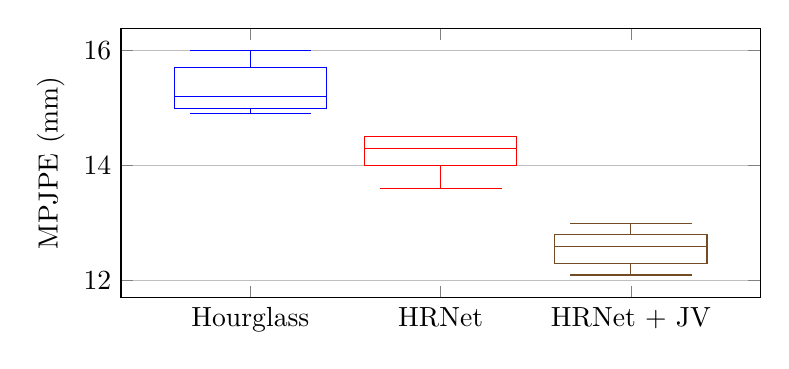
\begin{tikzpicture}
    \begin{axis}[
      boxplot/draw direction=y,
      width=0.8\linewidth, height=5cm,
      ylabel={MPJPE (mm)},
      xtick={1,2,3},
      xticklabels={Hourglass, HRNet, HRNet + JV},
      ymajorgrids
    ]
      \addplot+[boxplot prepared={
          draw position=1, lower whisker=14.9, lower quartile=15.0,
          median=15.2, upper quartile=15.7, upper whisker=16.0
        }] coordinates {};
      \addplot+[boxplot prepared={
          draw position=2, lower whisker=13.6, lower quartile=14.0,
          median=14.3, upper quartile=14.5, upper whisker=14.5
        }] coordinates {};
      \addplot+[boxplot prepared={
          draw position=3, lower whisker=12.1, lower quartile=12.3,
          median=12.6, upper quartile=12.8, upper whisker=13.0
        }] coordinates {};
    \end{axis}
  \end{tikzpicture}
  \caption{Per-joint MPJPE distribution.}
  \label{fig:mpjpe_box}
\end{figure}
\section{Discussion}
\textbf{Interpretation.} Both components contribute, and they are not redundant with one another. The backbone change accounts for the larger share of the improvement, which is consistent with the view that localisation of joints spanning only a few pixels is limited primarily by spatial resolution. The joint vector feature adds a further gain on top of an already high-resolution backbone, indicating that anatomical structure supplies information the network does not recover from appearance alone, and that a feature-level encoding is complementary to the loss-based regulariser rather than a substitute for it. In our runs the HRNet variants also reached the baseline's final error in roughly half the epochs, and per-joint error variance was lower with the joint vector feature.

\textbf{Limitations.} Four caveats bound these conclusions. (i) Our results are measured on a self-defined validation split rather than the official FreiHAND test server, so they establish relative ordering between the variants but not absolute standing (Section~\ref{subsec:setup}). (ii) $\lambda_{vec}$ requires tuning: too small and the term is inert, too large and absolute position accuracy is traded for vector consistency. (iii) The encoding infers occluded joints from visible neighbours and so degrades when several adjacent joints are occluded simultaneously, for instance an entire finger behind the palm. (iv) The adjacency graph is fixed, and monocular depth ambiguity is not resolved by bone-length constraints alone when multiple 3D configurations remain consistent with the image.

\textbf{Future work.} The immediate priority is a test-server submission under the official protocol, followed by evaluation on STB, InterHand2.6M and HO-3D to test whether the encoding transfers to stereo, interacting-hand and hand-object settings. Beyond that, replacing the fixed adjacency with learnable connectivity, and combining the high-resolution backbone with transformer-based relational modelling, are natural extensions.

\section{Conclusion}
In this work, we presented an enhanced framework for monocular 2D/3D hand pose estimation that combines a high-resolution feature extraction backbone with explicit modeling of anatomical relationships. By replacing the stacked Hourglass architecture with a High-Resolution Network (HRNet), the proposed method preserves fine-grained spatial information throughout the feature extraction process. In addition, the introduced joint vector feature encodes directional and length relationships between adjacent joints directly at the representation level, complementing standard heatmap-based pose estimation.
Experimental results on the FreiHAND benchmark demonstrate that these design choices lead to consistent improvements in both localization accuracy and structural coherence. Under a controlled comparison on a held-out validation split, the proposed approach improves PCK@20\,mm from 88\% to 93\% and reduces MPJPE from 15.2\,mm to 12.5\,mm relative to an Hourglass-based baseline trained under identical settings, while maintaining a modular and extensible architecture. Evaluation under the official FreiHAND test protocol remains to be carried out.
Both components are plug-and-play and add negligible inference cost, making them straightforward to graft onto existing heatmap-based pipelines.



% \section
% {Declarations}
% \subsection{Funding}
% The authors received no financial support for this research.
% \subsection{Conflicts of interest}
% The authors declare that they have no conflict of interest.
% \section*{Acknowledgments}
% We thank the authors of the original work available at \url{https://github.com/enghock1/Real-Time-2D-and-3D-Hand-Pose-Estimation} for their publicly released code.

\bibliographystyle{ACM-Reference-Format}
\bibliography{ICVGIP-Latex-Template}

\appendix



\end{document}